\documentclass[11pt]{scrartcl}

\usepackage[top=1.5cm]{geometry}
\usepackage{url}
\usepackage{float}
\usepackage{listings}
\usepackage{xcolor}
\usepackage{graphicx}

\setlength{\parindent}{0em}
\setlength{\parskip}{0.5em}

\newcommand{\youranswerhere}{[Your answer goes here \ldots]}
\renewcommand{\thesubsection}{\arabic{subsection}}

\lstdefinestyle{dbtsql}{
  language=SQL,
  basicstyle=\small\ttfamily,
  keywordstyle=\color{magenta!75!black},
  stringstyle=\color{green!50!black},
  showspaces=false,
  showstringspaces=false,
  commentstyle=\color{gray}}

\title{
  \textbf{\large Assignment 2} \\
  Query Tuning \\
  {\large Database Tuning}
}

\author{
  Group Name (e.g. A1, B5, B3) \\
  \large Peter Balint, 12213073 \\
  \large David Ottino, 51841010 \\
  \large Lukas Günter, 12125639
}

\begin{document}

\maketitle\thispagestyle{empty}

\subsection*{Creating Tables and Indexes}

SQL statements used to create the tables \texttt{Employee}, \texttt{Student}, and \texttt{Techdept}, and the indexes on the tables:

\begin{lstlisting}[style=dbtsql]
CREATE TABLE Employee (
    ssnum SERIAL PRIMARY KEY,
    name TEXT NOT NULL UNIQUE,
    manager INTEGER,
    dept TEXT,
    salary NUMERIC(10,2),
    numfriends INTEGER,
    FOREIGN KEY (manager) REFERENCES Employee(ssnum) ON DELETE SET NULL
);

CREATE UNIQUE INDEX idx_employee_ssnum ON Employee(ssnum);
CREATE UNIQUE INDEX idx_employee_name ON Employee(name);
CREATE INDEX idx_employee_dept ON Employee(dept);
\end{lstlisting}

\begin{lstlisting}[style=dbtsql]
CREATE TABLE Student (
    ssnum SERIAL PRIMARY KEY,
    name TEXT NOT NULL UNIQUE,
    course TEXT NOT NULL,
    grade CHAR(2)
);

CREATE UNIQUE INDEX idx_student_ssnum ON Student(ssnum);
CREATE UNIQUE INDEX idx_student_name ON Student(name);
\end{lstlisting}

\begin{lstlisting}[style=dbtsql]
CREATE TABLE Techdept (
    dept TEXT PRIMARY KEY,
    manager INTEGER,
    location TEXT,
    FOREIGN KEY (manager) REFERENCES Employee(ssnum) ON DELETE SET NULL
);

CREATE UNIQUE INDEX idx_techdept_dept ON Techdept(dept);
\end{lstlisting}

PostgreSQL automatically creates an index as soon as you put a UNIQUE contraint on a column. Therefore the indizes on ssnum and name would theoretically not be necessary, but we included them anyway for completness sake.


\subsection*{Populating the Tables}

The tables are filled using a Python script. We used CSV files as target files to store the table contents. The underlying data (employees, students, departments) was randomly generated, taking into account certain correlations and conditions - e.g. overlaps in people, manager assignments and department memberships.

\subsubsection*{TechDept}
For each technical department, we selected a randomly generated manager from the existing set of employees.

\begin{figure}[htbp]
    \centering
    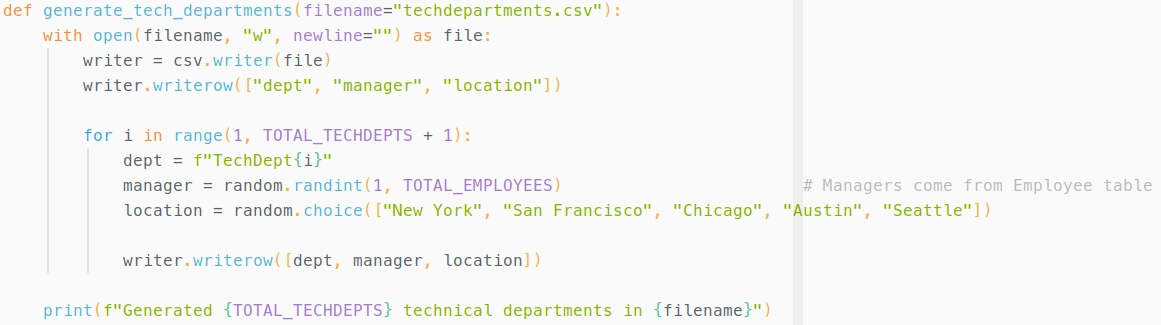
\includegraphics[width=0.8\textwidth]{Pics/TechDeptQuery.jpg}
    \caption{Script für Erstellung von TechDept}
    \label{fig:ScriptTechDept}
\end{figure}

\begin{figure}[htbp]
    \centering
    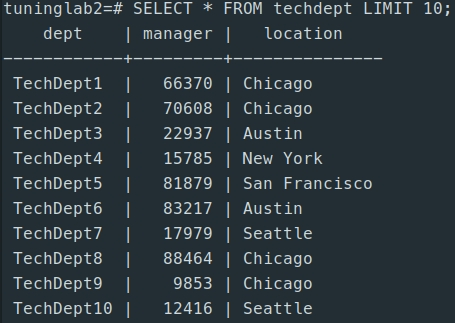
\includegraphics[width=0.8\textwidth]{Pics/TechDeptResult.jpg}
    \caption{Ergebnis TechDept}
    \label{fig:TechDeptResult}
\end{figure}

\subsubsection*{Students}

100,000 entries were generated for the student table. Each person received:

\begin{itemize}
    \item a unique social security number
    \item a unique name
    \item a random course and grade
\end{itemize}

\begin{figure}[htbp]
    \centering
    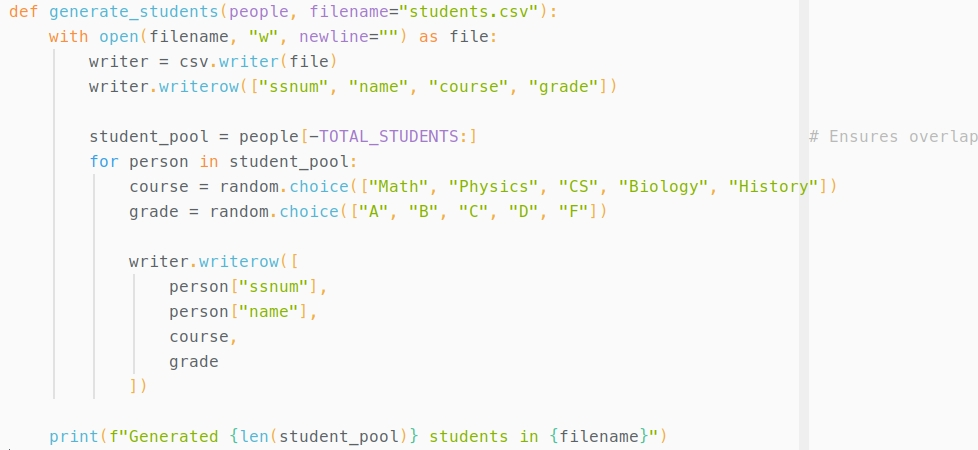
\includegraphics[width=0.8\textwidth]{Pics/StudentsScript.jpg}
    \caption{Script for creation of students}
    \label{fig:ScriptStudents}
\end{figure}

\begin{figure}[htbp]
    \centering
    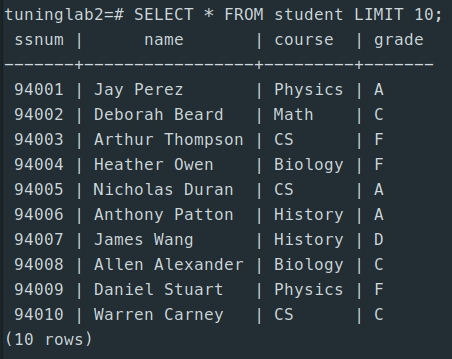
\includegraphics[width=0.8\textwidth]{Pics/StudentsResult.jpg}
    \caption{Excerpt from Students}
    \label{fig:StudentsResult}
\end{figure}

\subsubsection*{Employee}

100,000 entries were generated for the employee table. Each person received:

\begin{itemize}
    \item a unique social security number
    \item a unique name
    \item a random manager assignment
    \item with a 10 percent chance: an assignment to a technical departement
    \item random salary and amount of friends
\end{itemize}

\begin{figure}[htbp]
    \centering
    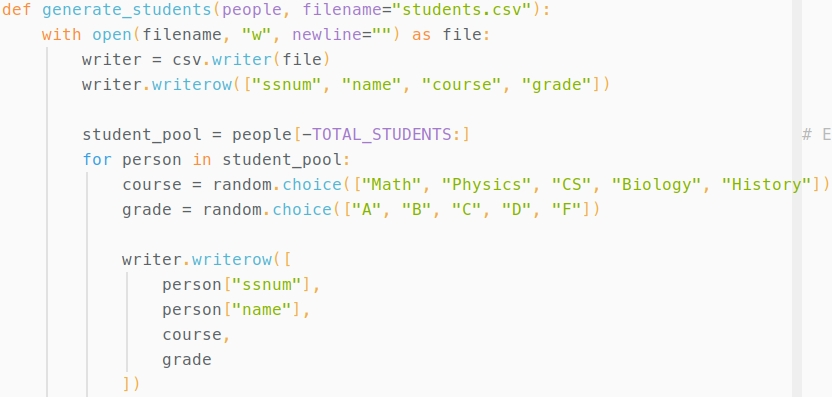
\includegraphics[width=0.8\textwidth]{Pics/ScriptEmployee.jpg}
    \caption{Script for creation of employees}
    \label{fig:ScriptEmployee}
\end{figure}

\begin{figure}[htbp]
    \centering
    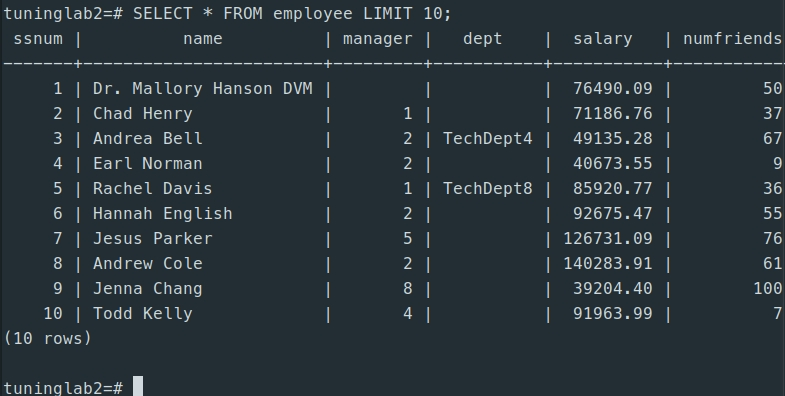
\includegraphics[width=0.8\textwidth]{Pics/EmployeeResult.jpg}
    \caption{Auszug aus Employee}
    \label{fig:EmployeeResult}
\end{figure}

\subsection*{Queries}

\subsubsection*{Query 1}

\paragraph{Original Query}

The first query shows the ssnum of all employees in tech-departments, that have a yearly salary within 1000 of the average salary over all tech-departments.

\begin{lstlisting}[style=dbtsql]
SELECT DISTINCT E1.ssnum
FROM Employee E1, Techdept T
WHERE E1.salary BETWEEN (
    (SELECT AVG(E2.salary)
     FROM Employee E2, Techdept T
     WHERE E2.dept = E1.dept
       AND E2.dept = T.dept) - 1000
) AND (
    (SELECT AVG(E2.salary)
     FROM Employee E2, Techdept T
     WHERE E2.dept = E1.dept
       AND E2.dept = T.dept) + 1000
);
\end{lstlisting}

\paragraph{Rewritten Query}

Give the rewritten query.

\begin{lstlisting}[style=dbtsql]
SELECT AVG(E.salary) as salary
FROM Employee E
JOIN Techdept T ON E.dept = T.dept;

SELECT DISTINCT E.ssnum
FROM Employee E
JOIN Techdept T ON E.dept = T.dept
WHERE E.salary BETWEEN salary - 1000 AND salary + 1000;
\end{lstlisting}

\paragraph{Evaluation of the Execution Plans}

Give the execution plan of the original query.

{\small
\parskip0pt\begin{verbatim}
Nested Loop Inner Join
	Seq Scan on employee as e1
	Filter: ((salary >= ((SubPlan 1) - '1000'::numeric)) AND (salary <= ((SubPlan 2) + '1000'::numeric)))
		Aggregate
			Nested Loop Inner Join
				Index Only Scan using idx_techdept_dept on techdept as t_1
				Index Cond: (dept = e1.dept)
				Bitmap Heap Scan on employee as e2
				Recheck Cond: (dept = e1.dept)
					Bitmap Index Scan using idx_employee_dept
					Index Cond: (dept = e1.dept)
		Aggregate
			Nested Loop Inner Join
				Index Only Scan using idx_techdept_dept on techdept as t_2
				Index Cond: (dept = e1.dept)
				Bitmap Heap Scan on employee as e2_1
				Recheck Cond: (dept = e1.dept)
					Bitmap Index Scan using idx_employee_dept
					Index Cond: (dept = e1.dept)
	Materialize
	Seq Scan on techdept as t
\end{verbatim}}

Nested Loop Inner Join: The tuples in Employee are read sequentially. This is restricted to the results of the two sub-queries SubPlan1 and SubPlan2. The result is then compared with TechDept and joined

SubPlan1/2: The index in TechDept on techdept is used to find all tech departments that correspond to the TechDept in Employee. The index on techdept in Employee is used for the comparison. This process is carried out twice, as the average earnings are used twice.

{\small
\parskip0pt\begin{verbatim}
Aggregate
	Hash Inner Join
	Hash Cond: (e.dept = t.dept)
		Seq Scan on employee as e
		Hash
			Seq Scan on techdept as t

Nested Loop Inner Join
	Seq Scan on employee as e
	Filter: ((salary >= '89008'::numeric) AND (salary <= '91008'::numeric))
	Memoize
		Index Only Scan using idx_techdept_dept on techdept as t
		Index Cond: (dept = e.dept)
\end{verbatim}}

Aggregate: Calculates a value based on all data records, in this case AVG(salary), based on a hash join.

Hash Inner Join: Employee is joined with TechDept. This is done with a hash join, so the values in both tables are read, then a hash table is created based on TechDept and compared with Employee.

Nested loop inner join: The values in Employee are read sequentially and only values with the corresponding salary are selected. These values are compared with TechDept, and the index on TechDept is also used and saved so that the index does not have to be run through several times for the same department.

Discuss, how the execution plan changed between the original and the rewritten query. In both the interpretation of the query plans and the discussion focus on the crucial parts, i.e., the parts of the query plans that cause major runtime differences.

In the naive query, two joins with one aggregate each are executed for each tuple in Employee, while after optimization the average value is calculated once and then reused.

\paragraph{Experiment}

\begin{table}[H]
  \centering
  \begin{tabular}{l|r}
    & Runtime [sec] \tabularnewline
    \hline
    Original query & 10.7524 seconds \tabularnewline
    Rewritten query & 0.2958 seconds \tabularnewline
  \end{tabular}
\end{table}

The improved query is significantly faster, as in the original query two joins and an aggregate have to be calculated for each tuple in Employee, which are very time-consuming and computationally intensive operations. The improved query calculates the value for the restriction in Employee once and then uses it again and again.

\subsubsection*{Query 2}

\paragraph{Original Query}

Give the second type of query that might be hard for your database to optimize.

\begin{lstlisting}[style=dbtsql]
SELECT ssnum
FROM Employee
WHERE dept IN (SELECT dept FROM Techdept)
\end{lstlisting}

\paragraph{Rewritten Query}

Give the rewritten query.

\begin{lstlisting}[style=dbtsql]
SELECT ssnum
FROM Employee, Techdept
WHERE Employee.dept = Techdept.dept
\end{lstlisting}

\paragraph{Evaluation of the Execution Plans}

{\small
\parskip0pt\begin{verbatim}
('Nested Loop  (cost=0.15..5212.39 rows=10007 width=4) (actual time=0.041..34.670 rows=10061 loops=1)',)
->  Seq Scan on employee  (cost=0.00..2723.00 rows=100000 width=14) (actual time=0.004..7.640 rows=100000 loops=1)',)
	->  Memoize  (cost=0.15..0.16 rows=1 width=10) (actual time=0.000..0.000 rows=0 	     loops=100000)',)
		  ->  	Index Only Scan using idx_techdept_dept on techdept  					(cost=0.14..0.15 rows=1 width=10) (actual time=0.004..0.004 rows=1 			loops=11)',)('Index Cond: (dept = employee.dept)',)
\end{verbatim}}

Nested Loop: For each employee, PostgreSQL checks if their dept exists in techdept, leading to many repeated sub-queries.

Seq Scan on employee: Scans the entire employee table row by row without using any index, which is slow for large datasets.

Memoize: Caches previous techdept lookups to avoid querying the same department multiple times, but still not optimal with many unique dept values.

Index Only Scan on techdept: Uses the index to check if the employee’s department exists, but this check is done 100,000 times.

{\small
\parskip0pt\begin{verbatim}
('Merge Join  (cost=1.56..1077.82 rows=10007 width=4) (actual time=0.070..5.647 rows=10061 loops=1)',)
 ->  Index Scan using idx_employee_dept on employee  (cost=0.29..9504.86 rows=100000 width=14) (actual time=0.028..4.032 rows=10062 loops=1)',)
	->  	Sort  (cost=1.27..1.29 rows=10 width=10) (actual time=0.040..0.042 rows=10 	      	loops=1)',)
		('        Sort Key: techdept.dept',)
		('        Sort Method: quicksort  Memory: 25kB',)
		->  	Seq Scan on techdept  (cost=0.00..1.10 rows=10 width=10) (actual 				time=0.008..0.009 rows=10 loops=1)
\end{verbatim}}

Merge Join: Combines rows from employee and techdept where the dept values match, using sorted input for efficient merging.

Index Scan on employee: Quickly retrieves employee rows by scanning the index to get sorted dept values.

Sort on Techdept: Sorts values to prepare them for the merge join.

Seq Scan on Techdept: Reads all rows from the small techdept table sequentially before sorting.

Naive Query: Does a sequential scan over all employee rows.

\begin{itemize}
\item For each row, it checks if dept is in techdept using index lookup.
\item Slower overall due to repeated subqueries.
\end{itemize}

Tuned Query: Uses Merge Join with:
\begin{itemize}
\item Index Scan on employee.dept
\item Sorted Scan on techdept
\item Optimizer uses indexes and sorting efficiently.
\item Much faster due to bulk processing and join strategy.
\end{itemize}


\paragraph{Experiment}

Give the runtimes of the original and the rewritten query.

\begin{table}[H]
  \centering
  \begin{tabular}{l|r}
    & Runtime [sec] \tabularnewline
    \hline
    Original query  & 0.1140 seconds \tabularnewline
    Rewritten query & 0.0814 seconds \tabularnewline
  \end{tabular}
\end{table}

Discuss, why the rewritten query is (or is not) faster than the original query.

In the naive query, a query is executed in TechDept for each tuple in Employee. The optimized query uses the existing indices efficiently and merges and filters the results in advance.

\paragraph{Differences between PostgreSQL and SQLite}

What differences did you observe between the postgres dbms and your alternative dbms?

\begin{table}[H]
  \centering
  \begin{tabular}{l|r|r|r}
    Query & Runtime SQLite (initial) & Runtime SQLite (full) \tabularnewline
    \hline
    Naive 1 & 0.897 seconds & 76.247 seconds \tabularnewline
    Tuned 1 & 0.077 seconds & 0.146 seconds \tabularnewline
    Naive 2 & 0.054 seconds & 0.104 seconds \tabularnewline
    Tuned 2 & 0.076 seconds & 0.074 seconds \tabularnewline
  \end{tabular}
\end{table}

SQLite uses a different execution model than PostgreSQL.  Instead of storing the execution plan as a tree, it generates a sequential bytecode representation which is directly executed.  The execution plan is a high-level description of this bytecode.

For query 1, significant runtime differences could be observed between the naive versions: SQLite managed to complete it in a tenth of the time when compared to PostgreSQL. However, further investigation revealed that this was only the initial execution time for the first row; retrieving all rows is in fact many times slower than in PostgreSQL.

To provide detailed query plans, we complied SQLite using the SQLITE\_ENABLE\_STMT\_SCANSTATUS option.  The plan for the naive query:

{\small
\parskip0pt\begin{verbatim}
QUERY PLAN (cycles=2427167766 [100%])
|--CORRELATED SCALAR SUBQUERY 1                                    (cycles=1682897569 [69%] loops=1159)
|  |--SEARCH T USING COVERING INDEX idx_techdept_dept (dept=?)     (cycles=1006677 [0%] loops=1159 rows=99 rpl=0.1 est=1.0)
|  `--SEARCH E2 USING INDEX idx_employee_dept (dept=?)             (cycles=1663633623 [69%] loops=99 rows=99192 rpl=1001.9 est=9.0)
|--CORRELATED SCALAR SUBQUERY 2                                    (cycles=739479704 [30%] loops=46)
|  |--SEARCH T USING COVERING INDEX idx_techdept_dept (dept=?)     (cycles=254716 [0%] loops=46 rows=46 rpl=1.0 est=1.0)
|  `--SEARCH E2 USING INDEX idx_employee_dept (dept=?)             (cycles=731309980 [30%] loops=46 rows=46482 rpl=1010.5 est=9.0)
|--SCAN E1 USING INDEX idx_employee_ssnum                          (cycles=9360875 [0%] loops=1 rows=1159 rpl=1159.0 est=983040.0)
`--SCAN T USING COVERING INDEX idx_techdept_dept                   (cycles=2448 [0%] loops=1 rows=1 rpl=1.0 est=1048576.0)
\end{verbatim}}

The plan itself largely resembles that of PostgreSQL.  A majority of the time is spent in looking up employees in an index for the dept column of employee.

The runtime difference is explained by the fact that we only retrieved the first row from the result, and SQLite's bytecode design allows for efficient evaluation of partial results.  Attempting to retrieve all rows inflates the execution time to 82 seconds, almost ten times \textit{slower} than PostgreSQL.

The tuned query reduces to two sequential scans over E, with a nested loop to find the corresponding tech department (if any):

{\small
\parskip0pt\begin{verbatim}
QUERY PLAN (cycles=105487554 [100%])
|--SCAN E                                                       (cycles=55791135 [53%] loops=1 rows=100000 rpl=100000.0 est=1048576.0)
`--SEARCH T USING COVERING INDEX idx_techdept_dept (dept=?)     (cycles=38080482 [36%] loops=100000 rows=10037 rpl=0.1 est=1.0)

QUERY PLAN (cycles=138855928 [100%])
|--SCAN E                                                       (cycles=76062419 [55%] loops=1 rows=100000 rpl=100000.0 est=983040.0)
`--SEARCH T USING COVERING INDEX idx_techdept_dept (dept=?)     (cycles=31517151 [23%] loops=100000 rows=10037 rpl=0.1 est=1.0)
\end{verbatim}}

For query 2, the runtime difference is less significant.  However, it yields another interesting result: the tuned version is \textit{slower} than the naive version.

Naive plan:

{\small
\parskip0pt\begin{verbatim}
QUERY PLAN (cycles=243576876 [100%])
|--USING INDEX idx_techdept_dept FOR IN-OPERATOR
`--SEARCH employee USING INDEX idx_employee_dept (dept=?)     (cycles=241322241 [99%] loops=1 rows=10037 rpl=10037.0 est=240.0)
\end{verbatim}}

Here, SQLite traverses an index on the techdept table's dept field, and searches for employees with according departments using an index on employee.

In contrast, the tuned plan looks like:

{\small
\parskip0pt\begin{verbatim}
QUERY PLAN
|--SCAN employee                                                       (loops=0 rows=0 rpl=NaN est=1048576.0)
`--SEARCH techdept USING COVERING INDEX idx_techdept_dept (dept=?)     (loops=0 rows=0 rpl=NaN est=1.0)
\end{verbatim}}

SQLite has decided to flip the looping order, doing a scan on the employee table and looking up the corresponding tech department for each employee.  It is interesting to contrast this with PostgreSQL's approach, which goes with a sort-merge join.  The reason for this discrepancy is that SQLite implements all joins as nested loops; it has no merge join strategy.

This time, we loaded the first 100 results, which the first query completes faster than the second query.  However, when loading \textit{all} results, the tuned query runs faster. (105ms vs 75ms).

A conclusion we can draw from this is that in SQLite, there may be a significant difference between the latency until the first row is returned and all rows are returned.

\subsection*{Time Spent on this Assignment}

Time in hours per person: \textbf{4}

\subsection*{References}

\begin{table}[H]
  \centering
  \begin{tabular}{l}
    \hline
    https://www.postgresql.org/docs/current/planner-optimizer.html \tabularnewline
    https://sqlite.org/draft/whybytecode.html \tabularnewline
    https://www.sqlite.org/optoverview.html\#joins \tabularnewline
    \hline
  \end{tabular}
\end{table}

\end{document}
